\documentclass{onrannual}

% provide additional characters
\usepackage{textcomp}

% Bibliography style; customize as appropriate, or remove if you don't use
% BibTeX or have no citations.
\usepackage[round]{natbib}
\setlength{\bibhang}{0pt}

% allow graphics inclusion
\usepackage{graphicx}

% for highlighting messages
\usepackage{color}

% optional: use hyperref to add in some PDF metadata
\hypersetup {
    pdftitle={Ocean Battlespace Sensing (OBS) S\&T Department Annual Report},
    pdfsubject={FY09 Annual Report},
    pdfauthor={First Author and Second Author},
    pdfkeywords={annual report, LaTeX, ONR}
}

%%
%% Two ways to specify an author.  Note the manual paragraph requirements if \affil is used.
%%

% \author{%
% First Author \\
% Academic Institute \\
% Laboratory 1 \\
% Somewhere, WA 11111 \\
% phone: (111) 222-3333    fax: (111) 222-4444     email: \href{mailto:first.author@ai.edu}{first.author@ai.edu}} \\
% 
% \and
%
% Second Author \\
% Government Institute \\
% Building 1234 \\
% Somewhere, WA 11112 \\
% phone: (111) 222-5555     fax: (111) 222-6666     email: \href{mailto:second.author@gi.gov}{second.author@gi.gov} \\
% }

\author{First Author}
\affil{%
Academic Institute \\
Laboratory 1 \\
Somewhere, WA 11111 \\
% NOTE: the trailing \\ is required at the end of this last line to separate authors
phone: (111) 222-3333    fax: (111) 222-4444     email: \href{mailto:first.author@ai.edu}{first.author@ai.edu} \\}

\author{Second Author}
\affil{%
Government Lab \\
Building 1234 \\
Somewhere, WA 11112 \\
phone: (111) 222-5555     fax: (111) 222-6666     email: \href{mailto:second.author@gl.gov}{second.author@gl.gov}} 

%% NOTE: distribution statements taken from 2009 guidance, and should be updated as appropriate for the current year.
%% One of these statements is required. so modify or uncomment as appropriate.
\distribution{DISTRIBUTION STATEMENT A: Distribution approved for public release; distribution is unlimited.}

%\distribution{DISTRIBUTION STATEMENT D: Distribution authorized to DoD components and U.S. DoD contractors only; Critical Technology; Dec 2009. Other requests for this document shall be referred to The Office of Naval Research (code 32). Destroy by any method that will prevent disclosure of contents or reconstruction of the document.}

% required
\title{Ocean Battlespace Sensing (OBS) S\&T Department Annual Report}

% required: always starts with N00014
\awardnumber{N00014-000-0000}

% optional
\projecturl{\url{http://www.onr.navy.mil/sci_tech/32/reports/annual/}}

%% Meat of the document goes here
\begin{document}
    
% The author prefers apalike, but it doesn't work when the year is missing.
% This causes problems for the fake citation used to show that the
% references section is optional.
\bibliographystyle{abbrvnat}

% print the title/author frontmatter
\maketitle

\section{LONG-TERM GOALS}
Briefly identify your top-level goals within which your effort exists. The goal of this \LaTeX{}
document class is to allow creation of annual reports matching the ONR requirements, without using a
commercial word processor.

\section{OBJECTIVES}
This section should contain the scientific or technological objectives of this effort.

\section{APPROACH}
Describe your proposed technical approach. Briefly identify the key individuals participating in this work at your own
or other organizations and the roles they play. In the present document, this section will describe the onrannual
document class.

The source \LaTeX{} file may be downloaded from
\href{http://mirror.ctan.org/macros/latex/contrib/onrannual/skeleton.tex}{CTAN}, and it is intended that you modify
it according to the comments within. In \TeX{} Live 2009, this file may also be found in the
\url{texmf-dist/doc/latex/onrannual} directory under the top-level \TeX{} Live install directory.
The onrannual class is a modification of the default article class, and including other styles may cause issues 
with spacing, particularly around section headings.

In the preamble, a few new commands may be used. The \verb=\awardnumber{N00014-000-0000}= macro is used to
define the award number, and the optional \verb=\projecturl{\url{http://foo.edu}}= is used to define a
project URL in the title block. ONR also requires a distribution statement to be inserted in the header
of the first page, and this is defined with the \verb=\distribution{xxx}= macro, where \verb=xxx= is replaced
with the appropriate text from the current ONR guidelines.

In general, the standard document macros may be used: \verb=\title{My Report Title}= is used to
set the title, and \verb=\maketitle= is used after \verb=\begin{document}= to display it.
Getting the author layout correct is slightly tricky, and one example is demonstrated here:
{
\scriptsize
\begin{verbatim}
\author{First Author}
\affil{%
Academic Institute \\
Laboratory 1 \\
Somewhere, WA 11111 \\
% NOTE: the trailing \\ is required at the end of this last line to separate authors
phone: (111) 222-3333    fax: (111) 222-4444     email: \href{mailto:first.author@ai.edu}{first.author@ai.edu} \\}
\end{verbatim}
}

This author and affiliation block is repeated for successive authors.
Standard \verb=\section= commands are used for sections, and \verb=\bibliography= may be
used to generate a bibliography. Subsections are not allowed, and will produce an error.

For other sample content to show usage of math and references, we can look at the 
Navier-Stokes equations, as given by \citet{Schlichting:2000}:

\begin{equation}
    \rho \frac{\partial D\overrightarrow{v}}{Dt} = \overrightarrow{f} - \mathrm{grad} p + \mathrm{Div} \tau
\end{equation}

with

\begin{equation}
    \tau = \mu \left(2\dot{\varepsilon} - \frac{2}{3}\delta \mathrm{div}\overrightarrow{v}\right)
\end{equation}

where $\delta$ is the Kronecker unit tensor $\left(\delta_{ij} = 1 for i = j, \delta_{ij} = 0 for i \neq j\right)$.

\section{WORK COMPLETED}
Actual tasks completed or technical accomplishments.

\section{RESULTS}
Describe meaningful technical results achieved in the report fiscal year. Make the significance clear. Emphasize what
was learned, not what was done. This should be a summary of significant results and conclusions, and, especially, any
``new capabilities'' generated.

\begin{figure}
    \begin{center}
        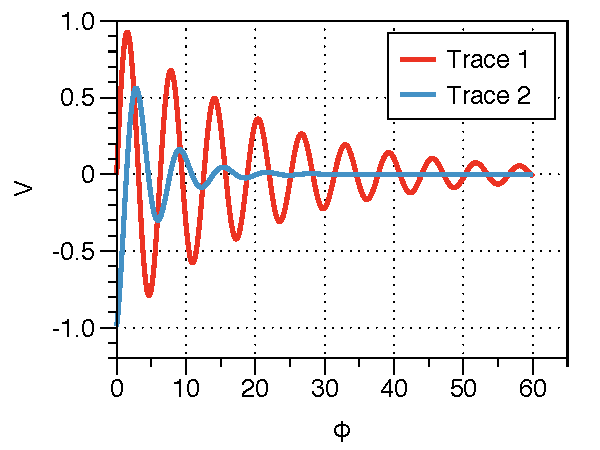
\includegraphics{samplefigure}
    \end{center}
    \caption{An example graphic. In general, you should use a long caption to describe the graphic in words. In this
    case, we use a long caption to ensure that all the caption text is correctly centered under the graphic.}
    \label{fig:label}
\end{figure}

Figure~\ref{fig:label} is a test graphic.

%%
%% If you use a large number of floats (figures or tables), you may want to issue a \clearpage
%% here to ensure that they're all flushed before the remaining sections. It's best to avoid
%% printing tables and figures in the middle of your bibliography, for instance, but sometimes
%% that's where they'd end up without manual intervention.
%%

\section{IMPACT/APPLICATIONS}
Potential future impact for science and/or systems applications

\section{TRANSITIONS}
An S\&T product has sufficiently matured and some organization (acquisition, industry, customer) outside of ONR is doing
something with it. ``Product'' includes equipment, prototypes, original ideas/theories, and equations. Include `who'
that `organization' is, how they are using it, and when it is expected to be used. It is of special interest if it is
already being used or has had acquisition funds committed. Examples are `products' entering acquisition, being used by
industry, or being used by other S\&T organizations such as DARPA).

%% If none, so state
\section{RELATED PROJECTS}
\textcolor{blue}{\textbf{If none, so state.}}
Identify closely related projects and briefly describe the nature of each relationship (include web links as
appropriate/available).

% This is a bibliography of all references cited in the report, assuming use of BibTeX
%% omit this section if there are none
\nocite{omitifnone} % hack to display the "omit..." text in the refs list
\bibliography{sample}

%% omit this section if there are none
\section{PUBLICATIONS}
\textcolor{blue}{\textbf{Omit if none.}}
Listing of publications produced during this effort. If you use Bib\TeX, you can use e.g., bibunits or multibib to
insert a second set of references, or just copy the contents of a .bbl file here.

%% omit this section if there are none
\section{PATENTS}
\textcolor{blue}{\textbf{Omit if none.}}
List all patent applications / awards for the project not reported in prior year's reports, or that have been previously
reported but whose status has changed. Note at end of item in brackets whether patent has been ``GRANTED'', for example:
``\ldots[granted]'', otherwise ``pending'' will be assumed.

%% omit this section if there are none
\section{HONORS/AWARDS/PRIZES}
\textcolor{blue}{\textbf{Omit if none.}}
List any received and not previously reported. Include recipient, recipient's institution, award `name', and award
sponsor.

\end{document}